% REMEMBER: You must not plagiarise anything in your report. Be extremely careful.

\documentclass{l4proj}
\usepackage {romannum}
\usepackage{tikz}
\usetikzlibrary{fit, matrix}
\usepackage{enumitem}
\usepackage{float}

%
% put any additional packages here
\usepackage{longtable}
%

\newcommand{\gethin}[1]{\marginpar{\footnotesize \color{red} {\bf GN:} \textsf{#1}}}

\begin{document}

%==============================================================================
%% METADATA
\title{String Matching Algorithm Visualisation Software}
\author{Michal Wozniak}
\date{\today}

\maketitle

%==============================================================================
%% ABSTRACT -  TO DO AT THE END
\begin{abstract}
Understanding string-matching algorithms can be a challenging task. Thus, the goal of the project is to implement a web application with a clear user interface, which will support students and enthusiasts learning about the Brute Force Approach, Boyer-Moore Horsepool and Knuth-Morris-Pratt algorithms. The product provides users with the capability to advance through animations and pseudocode while the execution is in progress, while also displaying the current variable values and explaining what is happening. The product also offers many quality-of-life features, such as mobile support to provide a seamless experience. The product has undergone a testing and evaluation phase, which has confirmed its correct functionality and ability to improve users' knowledge of string-matching algorithms.


    % Every abstract follows a similar pattern. Motivate; set aims; describe work; explain results.
    % \vskip 0.5em
    % ``XYZ is bad. This project investigated ABC to determine if it was better.
    % ABC used XXX and YYY to implement ZZZ. This is particularly interesting as XXX and YYY have
    % never been used together. It was found that
    % ABC was 20\% better than XYZ, though it caused rabies in half of subjects.''
\end{abstract}


% DONE
% \gethin{in the abstract why despite?}


% DONE - We will stick with string matching
% \gethin{abstract uses string matching while later it is string searching - be consistent, can mention the other but stick with one as the standard terminology}

%==============================================================================

% EDUCATION REUSE CONSENT FORM
% If you consent to your project being shown to future students for educational purposes
% then insert your name and the date below to  sign the education use form that appears in the front of the document.
% You must explicitly give consent if you wish to do so.
% If you sign, your project may be included in the Hall of Fame if it scores particularly highly.
%
% Please note that you are under no obligation to sign
% this declaration, but doing so would help future students.
%
\def\consentname {Michal Wozniak} % your full name
\def\consentdate {TO CHANGE} % the date you agree

\educationalconsent


%==============================================================================
\tableofcontents

%==============================================================================
%% Notes on formatting
%==============================================================================
% The first page, abstract and table of contents are numbered using Roman numerals and are not
% included in the page count.
%
% From now on pages are numbered
% using Arabic numerals. Therefore, immediately after the first call to \chapter we need the call
% \pagenumbering{arabic} and this should be called once only in the document.
%
% Do not alter the bibliography style.
%
% The first Chapter should then be on page 1. You are allowed 40 pages for a 40 credit project and 30 pages for a
% 20 credit report. This includes everything numbered in Arabic numerals (excluding front matter) up
% to but excluding the appendices and bibliography.
%
% You must not alter text size (it is currently 10pt) or alter margins or spacing.
%
%
%==================================================================================================================================
%
% IMPORTANT
% The chapter headings here are **suggestions**. You don't have to follow this model if
% it doesn't fit your project. Every project should have an introduction and conclusion,
% however.
%
%==================================================================================================================================
\chapter{Introduction}

% reset page numbering. Don't remove this!
\pagenumbering{arabic}


String search algorithms (otherwise known as string matching algorithms), such as Boyer-Moore (BM or BM Horsepool) and Knuth–Morris–Pratt (KMP) are blueprints typically introduced at the higher education level for computer scientists, as well as students of related degrees. Simply, these aim to find the exact sequence of words or characters in longer pieces of text. Although commonly taught and used within various pieces of software, it can be hard to develop an intuition for their inner working. I, myself, have had a hard time getting to grips with how these work, having been taught these in my COMPSCI4009 Algorithmics \Romannum{1} class in the School of Computing Science, University of Glasgow during the third year of my undergraduate degree.

Many computer applications exist to facilitate a visual way to show the steps of such algorithms, however there is potential to create a product that not only reduces the learning complexity but also provides a novel, mobile-friendly layout to help enthusiasts and students (such as me a few years ago) to get a good understanding of the aforementioned and similar algorithms.

This dissertation first aims to introduce the motivation behind the project,  explore existing software solutions and determine the high-level aims and requirements for the project. What follows is the development process outline, including design and implementation steps and decisions made for the application or project management. The penultimate chapter examines user perceptions of the product at various development stages \gethin{also testing in this chapter} before ultimately concluding its usefulness for the intended audience.


\section{Terminology And Notation}

Before discussing the project, it is important to highlight the terminology that will use throughout the dissertation, as it can differ between different institutions, text books and online documents.  The term \emph{pattern} will be used to refer to the \emph{sequence of words or characters we are searching for} and \emph{text} to denote the \emph{text we are searching within}. With regards to the algorithms, the Boyer-Moore algorithm will be referred to as "BM" and the Knuth-Morris-Pratt algorithm as "KMP", while for the Brute Force Algorithm the term "Naive Approach" will often be used.

\section{Motivation}

 % ubiquitous
 % anything with a computer

Although string matching algorithms are no longer the focus of today's development, \gethin{today's development?} they are crucial for people within the technology field to understand, since having such knowledge simplifies construction and maintenance of various software utilising these algorithms. \cite{GeeksforGeeks_2022} highlights some of the modern tools and fields employing them which includes the following. \gethin{add concrete references below}
%
\begin{itemize}
  \item
  \textbf{Plagiarism Detection.} String matching algorithms are used to compare the content of two documents to establish similarity. Such tools are used throughout most stages of education to ensure work originality. Such software will actually be used to check this paper for academic misconduct. \gethin{could mention turnitin?}
  \item
  \textbf{Spelling Checkers.} As with plagiarism detection, these can be particularly helpful in academia to ensure high-quality work.  \gethin{can here say more real world applications - everyone writing an email every day will use spell checking}
  \item
  \textbf{DNA Sequencing.} A lot of processes in the field of bioinformatics utilise string-matching facilities. One to highlight would be DNA pattern matching, which underpins gene analysis and helps determine potential illness, allowing for earlier and hence more effective treatment.
  \item
  \textbf{Digital Forensics.} Official public bodies aim to prevent crimes, with string matching playing a vital role in supporting investigations through performing information search on apprehended machines and law enforcement databases.
  \item
  \textbf{Spam Filters.} Used by email services to help determine email importance by looking for specific words.
  \item
  \textbf{Search Engines.} A ubiquitous tool used by the majority of people everyday, matching algorithms underpin this procedure for query processing.
  \item
  \textbf{Intrusion Detection Systems In Software.} In the cybersecurity field, we can analyse packets sent over a network by searching for malicious code based on known threats and malware.
\end{itemize}

The above list is not exhaustive and clearly there is a plethora of established tools using string matching algorithms, further making string matching algorithms foundational. This statement is supported ``\emph{by the wealth of published literature in this area} \citep{Stephen_1994}''. Most work today is based on the continued improvement of the performance of the information search process, due to the exponential increase of data available for analysis, as found by \cite{HASHEM201598} and his team while reviewing the rise of cloud computing. Therefore understanding of the current string matching algorithms is vital to being able to design new ones, but also to work with the vast amount of software using them. The developed application aims to ease the process of learning the workflow undertaken by the principal string matching algorithms, to help gauge a deep understanding that can benefit individuals in the future.


Despite the fact that the majority of current work is on optimisation and maintenance, even now these search algorithms are used to drive innovation. A recent example would be the Intelligent Predictive String Search Algorithm created by \cite{GURUNG2016161}, which eliminates the need for pre-processing and works based on comparing the first and last letter of the pattern acting as an extension to Boyer-Moore. Results show that it performs comparably to existing algorithms, at times better, while requiring less space and being simpler to understand. Another, more recent example would be the research conducted \cite{Ibrahim2023}, where two newly developed string matching algorithms had up to a 54\% performance increase compared to alternatives within the bio-informatics sphere.


\section{Initial High Level Requirements}
\label{intro:initial_requirements}


The project aim is to develop a product that can be used to help students develop an intuition on the working of algorithms from the COMSCI4009 Algorithmics \Romannum{1} course~\cite{algorithmics_1}. Following a discussion with the course coordinator at a time and looking into the objectives of a software engineering product, the following high-level goals (turned into user stories) have been established.
\begin{itemize}
  \item \textbf{Learning about the three string search algorithms included in the course.} As a user I want to be able to learn about string matching algorithms, including the naive approach, BM and KMP, so that I can pass the course.  \gethin{not pass the course but understand them?}
  \item \textbf{Animations.} As a user I want to be able to see how the string search algorithm of my choice behaves so that I can reproduce the way it works.
  \item \textbf{Clear UI.} As a user I want to be able to easily navigate and use the features of the product so that I can focus on the learning.
  \item \textbf{Documentation.} As a developer looking to improve the product, I want to be able to identify what each bit of code does quickly so that I can efficiently make required changes.
  \item \textbf{Tests.} As a user I want to be certain the product works as expected so that I am learning without distractions and the true behaviour of the algorithms.
\end{itemize}

These objectives are quite vague and open the software up to the developer's interpretation. To extract the wishes of the target audience I have decided to set up a requirement-gathering workshop, as discussed in \ref{intro:requirement_gathering_workshop}, but before doing so, to create material to discuss in the workshop, I explored existing solutions to see popular features, see Section~\ref{bac:existing_products}.


% Sequences consisting of symbols and words are fundamental to society in the modern world according to Graham \citet{Stephen_1994}, an individual who dedicated a whole book to discussing string search algorithms. He states that grouping those to construct strings is one of the most natural concepts to a human. Not only are strings key in everyday communication, but in everything we do - think of what you are doing right now, making a shopping list, looking at the time, there is an infinite number of uses we encounter every day without even thinking about them.  String matching algorithms are a layer above strings, but ``\emph{judging by the wealth of published literature in this area} \citep{Stephen_1994}'' these are just as foundational.

% Although no longer the focus of today's development, they are vital for people within the technology field to understand in depth, as the knowledge simplifies construction and maintainance of software utilising them. The importance of the necessity to understand is further intensified by the number of modern tools utilising string matching algorithms in various fields, as discussed in \citet{GeeksforGeeks_2022} and include the following.
% \begin{itemize}
%   \item \textbf{Plagiarism Detection.} String matching algorithms are used to compare the content of 2 documents to establish similarity. Such tools are used throughout most stages of education to ensure work originality.
% \item \textbf{Spelling Checkers.} As with plagiarism detection, these can be particularly helpful in academia to ensure high-quality, spotless work.
%   \item \textbf{DNA Sequencing.} A lot of processes in the field of bioinformatics utilise string-matching facilities. One to highlight would be DNA pattern matching, which underpins gene analysis and helps determine potential illness, allowing for earlier and hence more effective treatment.
%   \item \textbf{Digital Forensics.} Official public bodies aim to prevent crimes against society, with string matching playing a vital role in supporting investigations by aiding information search on apprehended machines and law enforcement databases.
%   \item \textbf{Spam Filters.} Used by email services to help determine email importance by looking for specific words.
%   \item \textbf{Search Engines.} Used by most people everyday, matching algorithms underpin this procedure for query processing.
%   \item \textbf{Intrusion Detection Systems In Software.} In the cybersecurity field, we can analyse packets sent over a network by searching for malicious code based on known threats and malware.
% \end{itemize}


\chapter{Background}

Based on the high-level goals for the project, it is important to introduce the string-matching algorithms that are essential for implementation within the product. This section will explore existing visualization solutions to determine how specific features have been implemented and what improvements can be made. The idea behind this is that non-functional prototypes will be developed that can be utilised in the requirement-gathering workshop.

\section{Principal String Matching Algorithms}
\label{bac:algorithms}

As mentioned, string-matching algorithms have the role of finding a specific sequence of symbols within a larger text. There exist several algorithms that have been developed over the years, each having its advantages and drawbacks. This section introduces three such algorithms: naive approach, Knuth-Morris-Pratt (KMP), and Boyer-Moore (BM), as per the initial requirements, see Section~\ref{intro:initial_requirements}.


\subsection{Brute Force Approach}
\label{bac:brute-force}

The brute force algorithm, also known as the naive approach, involves checking each pair of characters between the text and pattern until the solution is found. The pseudocode for such an algorithm is presented in Algorithm~\ref{alg:brute_force}.

\begin{algorithm}[t]
    \DontPrintSemicolon
    \KwData{$text$ // the text we are searching}
    \KwData{$pattern$ // the pattern we are searching for}

    \Begin{
      $\mathit{textLength} \longleftarrow $ length of text\;
      $\mathit{patternLength} \longleftarrow $ length of pattern\;
      $\mathit{startingPoint} \longleftarrow 0$\;
      $\mathit{patternIndex} \longleftarrow 0$\;
      $\mathit{textIndex} \longleftarrow 0$\;

      \While{$\mathit{startingPoint} \leq (\mathit{textLength} - \mathit{patternLength}) \;\; \&\& \; \; \mathit{patternIndex} < \mathit{patternLength}$}
      {
        \If{$\mathit{text}[\mathit{textIndex}] == \mathit{pattern}[\mathit{patternIndex}]$}
        {
           $\mathit{textIndex} \longleftarrow \mathit{textIndex} + 1$\;
           $\mathit{patternIndex} \longleftarrow \mathit{patternIndex} + 1$\;
        }
        \Else{
            $\mathit{patternIndex} \longleftarrow 0$\\
            $\mathit{startingPoint} \longleftarrow \mathit{startingPoint} + 1$ \\
            $\mathit{textIndex} \longleftarrow \mathit{startingPoint}$
        }
      }

    \If{$\mathit{patternIndex} == \mathit{patternLength}$} {
        return $\mathit{startingPoint}$
    }
    return $-1$

    }
\caption{Brute Force Algorithm}
\label{alg:brute_force}
\end{algorithm}

Starting from the $\mathit{startingPoint}$ of the text, we check each pair of text characters and pattern characters one by one (this happens by incrementing the $\mathit{textIndex}$ and $\mathit{patternIndex}$ upon a match, as shown by lines 9 and 10 respectively). If any pair of characters between the text and the pattern are not equal, we move one character forward in the text (completed by lines 14 and 15) and start checking from there against the start of the pattern (since we reset the $\mathit{patternIndex}$ to be 0, as of line 13).

Assuming a text of "string" and pattern of "sting" we can show the concept visually in Figure~\ref{alg:brute_force_exec}. In this example, our $startingPoint$ is 0, as we start comparing from the first character of the text. We then managed to match "st" between the text and the pattern, moving on to the comparison between "r" and "i" at the second index of both text and pattern. Here the characters don't match, so we increase our $staringPoint$ to start comparing text from index 1 to the pattern, in our example, we now start comparing from "t" in the text and the beginning of the pattern. Such process of moving one character forward in the text, upon each mismatch repeats until the text is exhausted (i.e. the $startingPoint$ is greater than the last index that could contain the pattern, as shown in line 7) or the pattern is fully matched (the $patternIndex$ is equal to $patternLength$, also on line 7).

\begin{figure}[t]
    \centering
    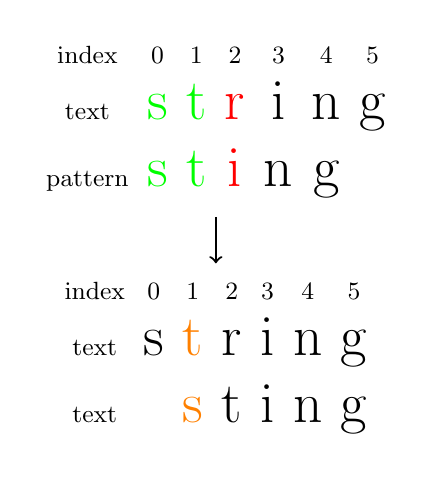
\begin{tikzpicture}
        [every node/.style={anchor=base, font=\huge},
        smallnum/.style={font=\small},
        textsize/.style={font=\small}]

        \begin{scope}
            \matrix (m) [matrix of nodes, nodes in empty cells]
            {
                |[textsize]| index &
                |[smallnum]|0 & |[smallnum]|1 &  |[smallnum]|2 &  |[smallnum]|3 &
                |[smallnum]|4 & |[smallnum]|5 \\
                |[textsize]| text & |[text=green]| s & |[text=green]| t &  |[text=red]| r &  i &
                n &  g \\
                |[textsize]| pattern & |[text=green]| s & |[text=green]| t &  |[text=red]| i & n &  g \\
            };
        \end{scope}

        \begin{scope}[yshift=-3cm]
            \matrix (m1) [matrix of nodes, nodes in empty cells]
            {
                |[textsize]| index &
                |[smallnum]|0 & |[smallnum]|1 &  |[smallnum]|2 &  |[smallnum]|3 &
                |[smallnum]|4 & |[smallnum]|5 \\
                |[textsize]| text &
                s & |[text=orange]| t &  r &  i &
                n & g \\
                |[textsize]| text & & |[text=orange]|s &  t & i & n &
                g \\
            };
        \end{scope}

        \draw[->,thick] (m.south) -- (m1.north);
    \end{tikzpicture}
    \caption{Example execution of the brute force algorithm.}
    \label{alg:brute_force_exec}
\end{figure}


The time complexity of this algorithm is $O(mn)$, assuming $n$ is the length of text and $m$ is the length of the pattern. This complexity arises from the fact that in the worst case (i.e., there is no match, but we will still need to compare the full length of the pattern when starting at each character of the text, as the mismatch always occurs on the last character of the pattern) we will need to go iterate over all characters in the text and all characters in the pattern at each $\mathit{startingPoint}$ value. The space complexity is constant ($O(1)$), as we only keep track of the $\mathit{startingPoint}$, $\mathit{patternIndex}$ and $\mathit{textIndex}$. Such an approach is trivial, \gethin{what is trivial?} however, it can form a basis for introducing the problem of searching large pieces of text efficiently and highlight the need for more sophisticated methods such as ones introduced in the following sections.


\subsection{Knuth-Morris-Pratt}

Knuth-Morris-Pratt greatly improves upon its predecessor described in Section~\ref{bac:brute-force} by achieving a linear time complexity of $O(m+n)$ in the worst case, paying for it with the increased space complexity of  $O(m)$ used to store pre-processing results. Created by Donald Knuth, Vaughan Pratt, and James H. Morris (see \cite{KMP}), it is an online algorithm published in 1977, which exploits a border table to avoid backtracking within the text, a phenomenon seen in the naive approach, as we move the $startingPoint$ value by 1, but we would have already looked further in the text to previously mismatch.  The pseudocode for the algorithm can be seen in Algorithm~\ref{alg:knuth_morris_pratt}.

\gethin{see changes I have made to brute force and do the same thing for the other algorithms}

\begin{algorithm}[H]
    \DontPrintSemicolon
    \KwData{$text$, The text we are searching. .}
    \KwData{$pattern$, The pattern we are searching for.}

    \Begin{
      $textLength \longleftarrow $ length of text\;
      $patternLength \longleftarrow $ length of pattern\;
      $patternIndex \longleftarrow 0$\;
      $textIndex \longleftarrow 0$\;

      $borderTable \longleftarrow $ createBorderTable(pattern)\;

      \While{$textIndex$ < $textIndex$}
      {
        \If{$text$[$textIndex$] == $pattern$[$patternIndex$]}
        {
           $textIndex \longleftarrow textIndex + 1$\;
           $patternIndex \longleftarrow patternIndex + 1$\;
           \If{$patternIndex == patternLength$} {return $textIndex - patternIndex$}
        }
        \Else{
            \If{$borderTable$[$patternIndex$] > 0}
            {
                $patternIndex$ = $borderTable$[$patterIndex$]
            }
            \Else{
                \If{$patternIndex == 0$}{
                    $textIndex \longleftarrow textIndex + 1$\;
                }
                \Else{
                    $patternIndex \longleftarrow 0$\;
                }
            }
        }
      }
      return $-1$
    }
\caption{Knuth-Morris-Pratt Algorithm}
\label{alg:knuth_morris_pratt}
\end{algorithm}


\subsubsection{Pre-Processing -- Line 6.}
The algorithm works based on having the border table tell the system which pattern character should be compared with the current text character at the next step so that we don't have to go backwards in the text. The border table is a data structure equal in length to the pattern, with each index representing a substring of the pattern up to, but excluding character at that index. For example in the string of "ababaca", the index of 4 assuming 0-indexing would consider the string of "ababa", but without the last character, as denoted by the red outline in Figure~\ref{fig:kmp-pre-process}. Each entry of the structure contains the size of the substring that is both a prefix and suffix of the substring considered. Considering our earlier example of index 4 the prefix and suffix would be ab, which has a length of 2, as the first two characters are ab and the last two characters are also ab, denoted in blue and orange respectively.

\begin{figure}[htp]
  \centering
  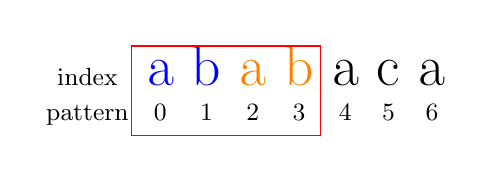
\begin{tikzpicture}
    [every node/.style={anchor=base, font=\huge},
     smallnum/.style={font=\small},
     textsize/.style={font=\small}]

    \matrix (m) [matrix of nodes, nodes in empty cells]
    {
      |[textsize]| index & |[text=blue]| a & |[text=blue]| b &  |[text=orange]| a & |[text=orange]| b & a & c & a \\
      |[textsize]| pattern & |[smallnum]| 0 & |[smallnum]| 1 & |[smallnum]| 2 & |[smallnum]| 3 & |[smallnum]| 4 & |[smallnum]| 5 & |[smallnum]| 6 \\
    };

    \node[fit=(m-1-2.north west) (m-2-5.south east), draw=red, inner sep=2pt] {};
  \end{tikzpicture}
  \caption{Working out border of pattern at index 4}
  \label{fig:kmp-pre-process}
\end{figure}


\gethin{add line numbers to subsubsections below?}

\subsubsection{Match.}
Upon a match, as with the brute force algorithm, we simply move one unit along within the text and the pattern, comparing the next pair of characters. This can be seen by lines 8 to 10 being the same as the naive approach match case.

\subsubsection{Mismatch.}
There are possible 3 cases for KMP to consider when we fail to match a pair of symbols. The cases are handled in the else clause spanning lines 15 to 27, a large chunk of the entire pseudocode. The case is determined based on the border table. More specifically we index the border table using the current index of the pattern we mismatched on - the $patternIndex$. If the border table reports a non-zero value, as checked by the conditional on line 16, it means the last $x$ characters in the already matched characters, match the start of the pattern, or rather the prefix of the matched pattern so far is also the suffix. In such case, we stay on the current character of the text, but shift the pattern to match the start of it with the last $x$ characters matched in the text/pattern. Visually this can be seen below, in Figure~\ref{kmp:mismatch-case-1}


\begin{figure}[hpt]
  \centering
  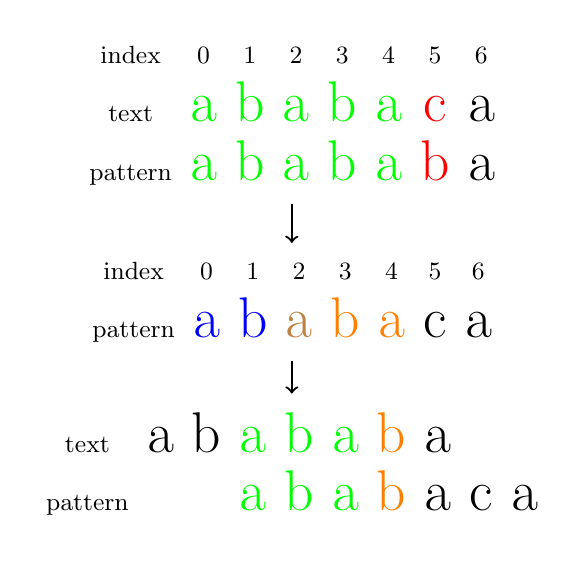
\begin{tikzpicture}
    [every node/.style={anchor=base, font=\huge},
     smallnum/.style={font=\small},
     textsize/.style={font=\small}]

    \begin{scope}
      \matrix (m1) [matrix of nodes, nodes in empty cells]
      {
        |[textsize]| index &
        |[smallnum]|0 & |[smallnum]|1 &  |[smallnum]|2 &  |[smallnum]|3 &
        |[smallnum]|4 & |[smallnum]|5 & |[smallnum]| 6 \\
        |[textsize]| text & |[text=green]| a & |[text=green]| b &  |[text=green]| a & |[text=green]| b &
        |[text=green]| a &
        |[text=red]|c & a \\
      |[textsize]| pattern & |[text=green]| a & |[text=green]| b &  |[text=green]| a & |[text=green]| b &
        |[text=green]| a &
        |[text=red]|b & a \\
      };

    \end{scope}

    \begin{scope} [yshift=-2cm]
    \matrix (m) [matrix of nodes, nodes in empty cells]
    {
       |[textsize]| index & |[smallnum]| 0 & |[smallnum]| 1 & |[smallnum]| 2 & |[smallnum]| 3 & |[smallnum]| 4 & |[smallnum]| 5 & |[smallnum]| 6 \\
      |[textsize]| pattern & |[text=blue]| a & |[text=blue]| b &  |[text=brown]| a & |[text=orange]| b & |[text=orange]| a & c & a \\
    };

    \draw[->,thick] (m1.south) -- (m.north);
    \end{scope}

    \begin{scope}[yshift=-4.2cm]
      \matrix (m2) [matrix of nodes, nodes in empty cells]
      {
        |[textsize]| text &  a &  b &  |[text=green]| a & |[text=green]| b &
        |[text=green]| a &
        |[text=orange]|b & a \\
        |[textsize]| pattern &
         &
         &
        |[text=green]| a & |[text=green]| b &  |[text=green]| a & |[text=orange]| b &
        a & c & a \\
      };
    \end{scope}

    \draw[->,thick] (m.south) -- (m2.north);

  \end{tikzpicture}
  \caption{KMP Mismatch Case 1 -- $borderTable$[$patternIndex$] is not 0}
  \label{kmp:mismatch-case-1}
\end{figure}


In this example, we mismatched the letters "c" and "b" on the $patternIndex$ of 5. The border of the substring of the pattern in the range $0..5$ exists, it being "aba", since the string starts with "aba" and finishes with "aba". In such case we now set the $patternIndex$ to 3, shifting it right in relation to the text.  We continue checking from the "b" in both text and pattern.

In the case the $borderTable$ reports a value of 0, we need to also consider the $patternIndex$ value. Should the currently checked character in the pattern be the very first character, we essentially perform the naive approach step, moving one character forward in the text (shown by the increment on line 21). We now compare the pattern from the next character in the text: \gethin{reference figure or algorithm}


\begin{figure}[H]
    \centering
    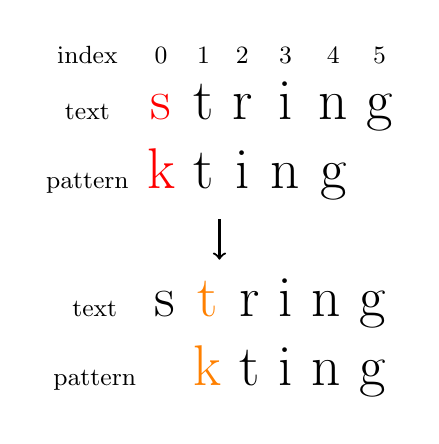
\begin{tikzpicture}
        [every node/.style={anchor=base, font=\huge},
        smallnum/.style={font=\small},
        textsize/.style={font=\small}]

    \begin{scope}
      \matrix (m) [matrix of nodes, nodes in empty cells]
      {
        |[textsize]| index &
        |[smallnum]|0 & |[smallnum]|1 &  |[smallnum]|2 &  |[smallnum]|3 &
        |[smallnum]|4 & |[smallnum]|5  \\
        |[textsize]| text &  |[text=red]|  s &  t &  r &  i &
         n &  g \\
      |[textsize]| pattern & |[text=red]| k & t &  i & n &  g \\
      };

    \end{scope}

     \begin{scope}[yshift=-2.5cm]
      \matrix (m1) [matrix of nodes, nodes in empty cells]
      {
        |[textsize]| text &
        s & |[text=orange]| t &  r &  i &
        n & g \\
      |[textsize]| pattern && |[text=orange]| k &  t &  i & n &
        g \\
      };
    \end{scope}

    \draw[->,thick] (m.south) -- (m1.north);
    \end{tikzpicture}
    \caption{KMP Mismatch Case 2 -- both $borderTable$[$patternIndex$] and $patternIndex$ are 0 }
    \label{kmp:mismatch-case-2}
\end{figure}


Should be currently checked value in the pattern not be the first character, we simply start the comparison again from the current $textIndex$ by resetting the $patternIndex$, as shown by line 24. This is similar to the naive approach, but we don't move to the next character from the $startingPoint$, but restart the comparison with mismatched character in the text. Such case is show visually in Figure~\ref{kmp:mismatch-case-3}.


\begin{figure}[H]
    \centering
    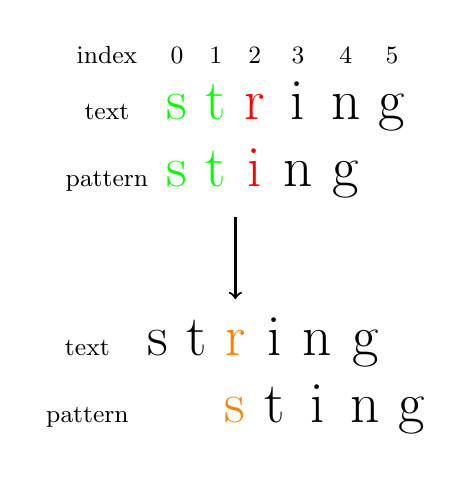
\begin{tikzpicture}
        [every node/.style={anchor=base, font=\huge},
        smallnum/.style={font=\small},
        textsize/.style={font=\small}]

    \begin{scope}
      \matrix (m) [matrix of nodes, nodes in empty cells]
      {
        |[textsize]| index &
        |[smallnum]|0 & |[smallnum]|1 &  |[smallnum]|2 &  |[smallnum]|3 &
        |[smallnum]|4 & |[smallnum]|5  \\
        |[textsize]| text & |[text=green]| s & |[text=green]| t &  |[text=red]| r &  i &
         n &  g \\
      |[textsize]| pattern & |[text=green]| s & |[text=green]| t &  |[text=red]| i & n &  g \\
      };

    \end{scope}

     \begin{scope}[yshift=-3cm]
      \matrix (m1) [matrix of nodes, nodes in empty cells]
      {
        |[textsize]| text &
         s & t &  |[text=orange]| r &  i &
        n & g \\
      |[textsize]| pattern & & & |[text=orange]| s &  t &  i & n &
        g \\
      };
    \end{scope}

    \draw[->,thick] (m.south) -- (m1.north);
    \end{tikzpicture}
    \caption{KMP Mismatch Case 3 -- $borderTable$[$patternIndex$] is 0, but $patternIndex$ is not}
    \label{kmp:mismatch-case-3}
\end{figure}

Above is the same example as in Figure \ref{alg:brute_force_exec}, however this time instead of starting checking from index 1 in the text, we start checking from index 2, as there is no border - we avoid going back to index 1 in the text, as we have already been there previously and know it cannot match "r" there.


\subsection{Boyer-Moore Algorithm Horsepool}

Boyer-Moore is an algorithm introduced in 1975, as summarised by \cite{bm}, before the dawn of KMP. On paper it appears slower than its ancestor, as its worst time complexity is $O(nm)$, however, it has been found that its performance is almost always better in practice. The reason for such a phenomenon is the fact BM is prone to skipping many characters per step, quickly eliminating areas of the text that cannot possibly match the pattern. Recently \cite{KMPvsBM} showed that BM outperformed KMP almost every single time, in some cases reaching one-third of the time it takes KMP to run.

Similar to KMP, the algorithm utilises a pre-processing data structure, which determines the next comparison during execution. Unlike the 2 previous algorithms, it works based on comparing right to left, starting the comparison from the last character in the pattern to the corresponding character in the text. There exist many variations, however, for this project, the focus was the Horsepool variant, a version using the "bad-character" rule only, as opposed to both the "bad-character" and "good-suffix" rules. It is important to note that the horsepool variant is more commonly used as the original algorithm provides little to no performance benefits \cite{horsepool_vs_full}, specifically due to little impact from the good-suffix rule. The pseudocode for the variant is as follows:


\begin{algorithm}[H]
    \DontPrintSemicolon
    \KwData{$text$, The text we are searching. .}
    \KwData{$pattern$, The pattern we are searching for.}

    \Begin{
      $textLength \longleftarrow $ length of text\;
      $patternLength \longleftarrow $ length of pattern\;
      $startingPoint \longleftarrow 0$\;
      $patternIndex \longleftarrow patternLength - 1$\;
      $textIndex \longleftarrow patternLength - 1$\;

      $lastOccurrenceTable \longleftarrow $ createLastOccurrenceTable(pattern)\;

      \While{$startingPoint$ <= ($textLength$ - $patternLength$) $\&\&$ $patternIndex$ >= $0$}
      {
        \If{$text$[$textIndex$] == $pattern$[$patternIndex$]}
        {
           $textIndex \longleftarrow textIndex - 1$\;
           $patternIndex \longleftarrow patternIndex - 1$\;
           \If{$patternIndex == patternLength$} {return $textIndex - patternIndex$}
        }
        \Else{
            $startingPoint \longleftarrow startingPoint + max(1, patternIndex  - lastOccurrenceTable[text[textIndex]])$\;
            $textIndex \longleftarrow textLength - min(patternIndex, 1  + lastOccurrenceTable[text[textIndex]])$\;
            $patternIndex \longleftarrow pattenLength - 1$\;
        }
      }
      \If{$patternIndex$ < $0$} {
        return $startingPoint$
      }
      return $-1$
    }
\caption{Boyer-Moore Algorithm}
\label{alg:boyer_moore}
\end{algorithm}


\subsubsection{Pre-Processing and The Bad Character Rule} On line 7, the execution context is changed to a function that creates a dictionary of the last occurrence. As mentioned this is a data structure, which supports the algorithm during execution by storing the last index of each character in the pattern. For example in the word "ababa", the last occurrence would look as follows:
\begin{itemize}
    \item{a : 4}
    \item{b : 3}
\end{itemize}


\subsubsection{Match} Upon a match, lines 10 and 11 show $textIndex$ and $patternIndex$ are both decreased. This is due to the fact we check right to left, instead of left to right, meaning characters to the right are already matched.

\subsubsection{Mismatch} Upon a mismatch, there are 3 possible things that can happen during execution.  In the first case the last occurrence of mismatched character in text has not been matched yet i.e. the last occurrence exists to the left of currently checked pattern character. In such situation, we need to shift the pattern in such way to line up the last occurrence with the current text element we are looking at.  Referring to example in Figure~\ref{bm:mismatch-case-1}, we need the "a" in the pattern to be moved to the right until lined up with the mismatched a in the test.

\begin{figure}[H]
  \centering
  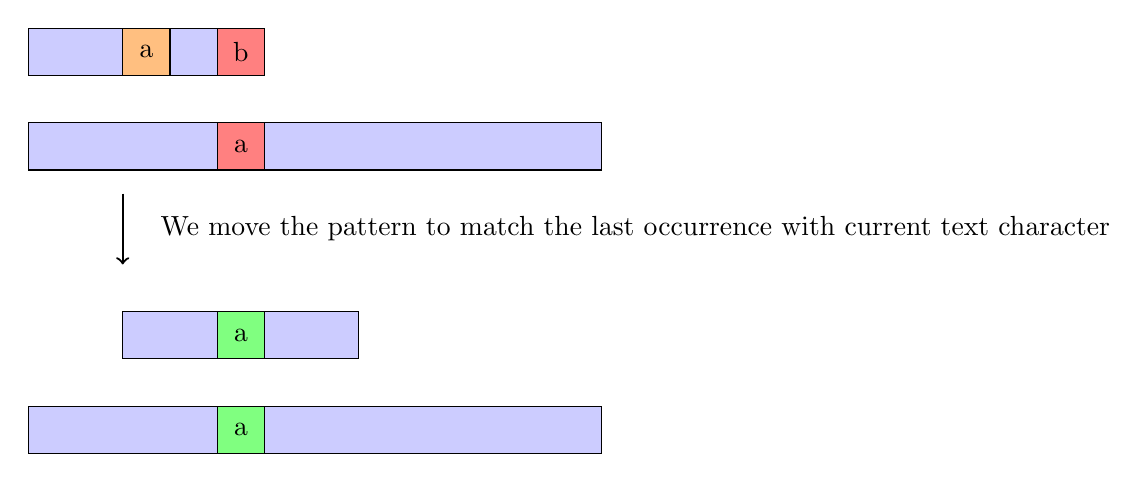
\begin{tikzpicture}[scale=0.6]
    \begin{scope}
        \draw [draw=black, fill=blue!20] (0,0) rectangle (4,1);
        \draw [draw=black, fill=red!50] (4, 0) rectangle (5, 1) node[midway] {b};;
        \draw [draw=black, fill=orange!50] (2,0) rectangle (3,1) node[midway] {a};
        \draw [draw=black, fill=blue!20] (0, -2) rectangle (\textwidth, -1);
        \draw [draw=black, fill=red!50] (4, -2) rectangle (5, -1) node[midway] {a};;
    \end{scope}

    \draw[->, thick] (2, -2.5) -- (2, -4)  node[midway, right, xshift=10pt] {We move the pattern to match the last occurrence with current text character};

    \begin{scope}
        \draw [draw=black, fill=blue!20] (2,-6) rectangle (7,-5);
        \draw [draw=black, fill=green!50] (4,-6) rectangle (5,-5) node[midway] {a};;
        \draw [draw=black, fill=blue!20] (0, -8) rectangle (\textwidth, -7);
        \draw [draw=black, fill=green!50] (4, -8) rectangle (5, -7) node[midway] {a};;
    \end{scope}
  \end{tikzpicture}
  \caption{Boyer-Moore Mismatch Case 1}
  \label{bm:mismatch-case-1}
\end{figure}


With case 2, the last occurrence of the mismatched character has already been matched i.e the last occurrence is to the right of currently checked pattern character. In such case we simply move the pattern one place forward respective to the text (increment the $textIndex$ by 1 )and restart the search from the end of the string. This happens because we cannot guarantee no match, since there could be another instance of the character within the pattern to match the text, one that is not the last occurrence. Figure \ref{bm:mismatch-case-2} shows such case.

\begin{figure}[H]
  \centering
  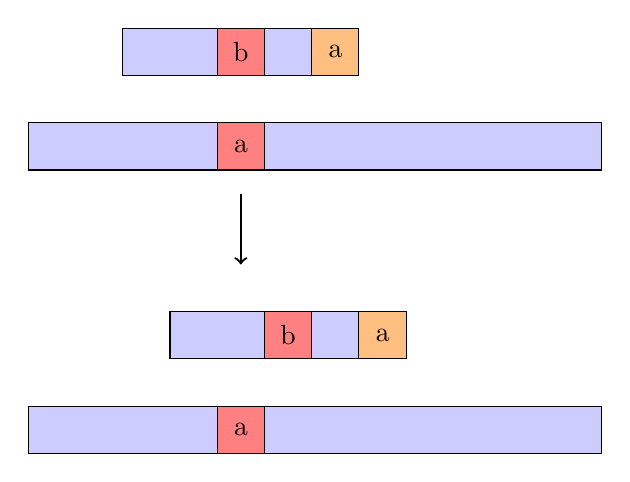
\begin{tikzpicture}[scale=0.6]
    \begin{scope}
        \draw [draw=black, fill=blue!20] (2,0) rectangle (7,1);
        \draw [draw=black, fill=red!50] (4, 0) rectangle (5, 1) node[midway] {b};;
        \draw [draw=black, fill=orange!50] (6,0) rectangle (7,1) node[midway] {a};
        \draw [draw=black, fill=blue!20] (0, -2) rectangle (\textwidth, -1);
        \draw [draw=black, fill=red!50] (4, -2) rectangle (5, -1) node[midway] {a};;
    \end{scope}

    \draw[->, thick] (4.5, -2.5) -- (4.5, -4); % Centering the arrow horizontally

    \begin{scope}
        \draw [draw=black, fill=blue!20] (3,-6) rectangle (8,-5);
        \draw [draw=black, fill=red!50] (5,-6) rectangle (6,-5) node[midway] {b};;
        \draw [draw=black, fill=orange!50] (7,-6) rectangle (8,-5) node[midway] {a};
        \draw [draw=black, fill=blue!20] (0, -8) rectangle (\textwidth, -7);
        \draw [draw=black, fill=red!50] (4, -8) rectangle (5, -7) node[midway] {a};;
    \end{scope}

  \end{tikzpicture}
  \caption{Boyer-Moore Mismatch Case 2}
  \label{bm:mismatch-case-2}
\end{figure}


The final case covers the situation where there is  no last occurrence for a text character, simply the character does not appear in the pattern. In such case we we move the pattern past the mismatched element i.e. we start checking the text from the next element, as it is impossible to match any substring where the pattern character does not exist. Visually this can be seen as:

\begin{figure}[H]
  \centering
  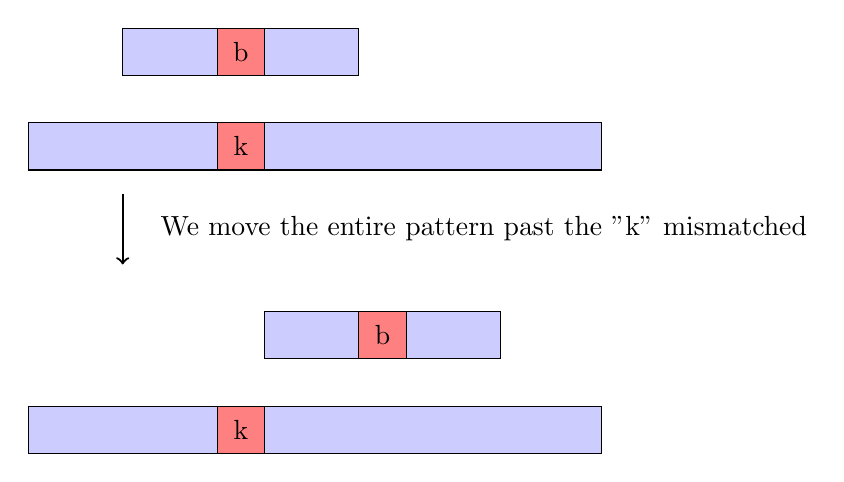
\begin{tikzpicture}[scale=0.6]
    \begin{scope}
        \draw [draw=black, fill=blue!20] (2,0) rectangle (7,1);
        \draw [draw=black, fill=red!50] (4, 0) rectangle (5, 1) node[midway] {b};;
        \draw [draw=black, fill=blue!20] (0, -2) rectangle (\textwidth, -1);
        \draw [draw=black, fill=red!50] (4, -2) rectangle (5, -1) node[midway] {k};;
    \end{scope}

    \draw[->, thick] (2, -2.5) -- (2, -4)  node[midway, right, xshift=10pt] {We move the entire pattern past the "k" mismatched};


    \begin{scope}
        \draw [draw=black, fill=blue!20] (5,-6) rectangle (10,-5);
        \draw [draw=black, fill=red!50] (7,-6) rectangle (8,-5) node[midway] {b};;
        \draw [draw=black, fill=blue!20] (0, -8) rectangle (\textwidth, -7);
        \draw [draw=black, fill=red!50] (4, -8) rectangle (5, -7) node[midway] {k};;
    \end{scope}

  \end{tikzpicture}
  \caption{Boyer-Moore Mismatch Case 3}
  \label{bm:mismatch-case-3}
\end{figure}


The 3 cases combined make up the algorithm, over the years the 3 cases have been optimised to 3 variable equations defined between lines 17-19, which won't be explained here, but for more information, refer to this resource \cite{}.


\section{Existing Products}
\label{bac:existing_products}

There exists a plethora of software applications made and published to educate in regards to  string-matching algorithms. Each solution takes a different approach to the design of the software application. Some focus more on creating a visually appealing and user-friendly interface, while others prioritize the functionality and features of the application. Ultimately, the approach taken depends on the target audience's needs and experiences as well as the goals of the project. This section will summarise the solutions explored, discuss the advantages and disadvantages of each and concluding with the details that will be use within the prototypes of the requirement-gathering workshop. The features chosen can be seen in wireframes 1 through to 3 in Appendix~\ref{app:initial_wireframes}.

\subsection{\href{https://cmps-people.ok.ubc.ca/ylucet/DS/Algorithms.html}{Data Structure Visualizations}}

The original Java-based version of this application was developed by David Galles of the University of San Francisco in 2011, however the current website Flash-based version is an updated application developed by Yves Lucet of I. K. Barber School of Arts \& Sciences, UBC Okanagan. The application contains visualisers for algorithms from a range of areas, not only string-matching, including, for example, Heap-related algorithms. The range of applcaitions makes the application useful for any Computer Science student, teacher, professional or enthusiast.  Being ranked quite highly on the search engine results suggests it is also a very popular visualiser enjoyed by many people --making it a defacto product for analyse.

Advantages of this applcation:
\begin{itemize}
    \item \textbf{Custom text and pattern.} It is possible to execute the algorithms with custom text and pattern, making it possible to adapt the execution to the user's case.
    \item \textbf{"Failure function" building for KMP.}  The visualiser shows how the preprocessing steps for KMP are completed, albeit a different method to the one in Algorithmics \Romannum{1}.
    \item \textbf{Reset.} The site can reset everything to default values, always giving the user an out when something is going wrong - in line with usability heuristic number 3, created by \cite{Nielsen_2024}, by giving users an "emergency exit".
    \item \textbf{Stepping forward and backward.} The user can step forward and backwards one step at a time.
    \item \textbf{Skipping to first and last step.} The user can go all the way to the start or the end should they wish.
    \item \textbf{Pause/Play.} The user can pause execution and later resume it.
    \item \textbf{Animation Speed.} It is possible to change how quickly the animation goes through the steps.
    \item \textbf{Canvas size change.}  The site gives the ability to set the canvas size to exact measurements wished by the user.
    \item \textbf{Change control location.} A quality-of-life feature, where the user can place the control dashboard either as a header or a footer.
    \item \textbf{Addition of new algorithm.} There is a guide, which can be followed to add a new algorithm to visualise.
\end{itemize}


Disadvantages of the application:
\begin{itemize}
    \item \textbf{Cannot reset while running.} The visualizer controls are not very intuitive. You can only reset at the final step, and using the skip functionality sometimes crashes the site.
    \item \textbf{Out-of-date aesthetics.} The website looks quite dated, which may put off some users from using it and instead looking for an alternative.
    \item \textbf{Difficult to follow tutorial.} The tutorial is quite involved and requires some understanding of the massive codebase. While possible, it is not easy to add a new algorithm.
    \item \textbf{Difficult to read certain elements.} The animation is never resized, hence some elements can be difficult to read, especially on larger displays.
    \item \textbf{Not mobile-friendly.} Although the animation is fairly visible, a horizontal scroll is required to access all control elements on a smaller screen.
    \item \textbf{Lacking the Brute Force Algorithm.} No animations for the naive approach are implemented at all.
\end{itemize}


% \begin{longtable}{|p{0.45\linewidth}|p{0.45\linewidth}|}
% \hline
% \textbf{Advantages} & \textbf{Disadvantages} \\ \hline
% \endhead
% \begin{itemize}[leftmargin=*]
%     \item \textbf{Custom text and pattern}: It is possible to execute the algorithms with custom text and pattern.
%     \item \textbf{"Failure function" building for KMP}: The visualiser shows how the preprocessing steps for KMP are completed, albeit a different method to the one in Algorithmics \Romannum{1}.
%     \item \textbf{Reset}: The site has the ability to reset everything to default values, always giving the user an out when something is going wrong.
%     \item \textbf{Stepping forward and backward}: The user is able to step forward and backward one step at a time.
%     \item \textbf{Skipping to first and last step}: The user is able to go all the way to the start or the end should they wish.
%     \item \textbf{Pause/Play}: The user is able to pause execution and later resume it.
%     \item \textbf{Animation Speed}: It is possible to change how quickly the animation goes through the steps.
%     \item \textbf{Canvas size change}: The site gives the ability to set the canvas size to exact measurements wished by the user.
%     \item \textbf{Change control location}: A quality of life feature, where the user can place the control dashboard either as a header or a footer.
%     \item \textbf{Addition of new algorithm}: There is a guide, which can be followed to add a new algorithm to visualize.
% \end{itemize} &
% \begin{itemize}[leftmargin=*]
%     \item \textbf{Cannot reset while running}: The controls are quite clunky when the visualiser is running. It is only possible to reset when reaching the final step. I also found sometimes using the skip functionality breaks the entire site, forcing the user to reload.
%     \item \textbf{Out-of-date aesthetics}: The website looks quite dated, which may put off some users from using it and instead looking for an alternative.
%     \item \textbf{Difficult to follow tutorial for extension}: The tutorial is quite involved and requires some understanding of the massive codebase.
%     \item \textbf{Difficult to read certain elements}: The animation is never resized, hence some elements can be difficult to read, especially on larger displays.
%     \item \textbf{No mobile-friendly}: Although the animation is fairly visible, a horizontal scroll is required to access all control elements.
% \end{itemize} \\ \hline
% \end{longtable}

Overall the product does a great job at educating via great animations for a wide range of algorithms, also providing a vast spectrum of quality-of-life features, attempting to make the learning process as frictionless for the user as possible. However the product is also quite dated and several features of the app are not functioning smoothly, some appearing to be causing crashes on the site. The UI experience is hence not optimal, likely causing the user to look for an alternative learning tool. For my wireframes, I decided to implement a version of the animation style (the use of squares and highlighting of their border), as well as the pause/play, go forward, go backwards and the animation speed setter features, as I thought all of these made it easier to understand the KMP and BM algorithms.

\subsection{\href{https://algorithm-visualizer.org/}{Algorithm Visualizer}}

Another website that holds a large selection of algorithms and concepts to visualise, however, it adds a modern spin onto the UI design, as well as providing a lot of quality-of-life features to the user.   It is an open-source effort, where anyone can add a new visualisation.

Advantages of the application:
\begin{itemize}
    \item \textbf{Custom text and pattern.} It is possible to execute the algorithms with custom text and pattern.
    \item \textbf{Border table building for KMP.}  The visualiser shows how the preprocessing steps for KMP are completed, utilising the same concepts as in Algorithmics \Romannum{1}.
    \item \textbf{Reset.} The site can reset everything to default values, always giving the user an out when something is going wrong.
    \item \textbf{Stepping forward and backward.} The user can step forward and backwards one step at a time.
    \item \textbf{Setting exact step.} The platform provides a range element, which can be toggled to any step in the execution.
    \item \textbf{Pause/Play.} The user can pause execution and later resume it.
    \item \textbf{Animation Speed.} It is possible to change how quickly the animation goes through the steps.
    \item \textbf{Animation size change.}  The scroll-wheel of the mouse can be used to zoom into the animation, should anything not be visible.
    \item \textbf{Seperate and resizeable canvases.} Separate UI elements are used to show preprocessing steps and the actual algorithm execution - making it easy to tell what is doing what. On top of this, each is resizeable, allowing users to place focus on whatever part they struggle to understand.
    \item \textbf{Addition of new algorithms.} There is a guide and custom library, which can be utilised to add a new algorithm. This can even be done on the online platform itself - acting as an online code editor.
    \item \textbf{Source code on Github.} The source code is located on Github so that it can be easily forked or modified by anyone to meet their wishes.
    \item \textbf{Algorithm Description} Contains basic information about the algorithm in a README file, as well as the complexity.
    \item \textbf{Psuedocode Highlighting.} The animation is accompanied by the pseudocode, which is highlighted according to the step currently on.
    \item \textbf{Full screen} The UI allows the user to go full screen with the animation, on top of being able to hide the pseudocode if required.
    \item \textbf{Sign-In.} The site has a sign-in feature integration via Github, allowing changes to be made on your account e.g. visualisation of a new algorithm.
\end{itemize}


Disadvantages of the application:
\begin{itemize}
    \item \textbf{Unclear execution.} I have noticed that the animations on the website are difficult to comprehend. The pattern is not displayed clearly concerning the text being searched, and there are no descriptive messages to explain the current execution state.
    \item \textbf{No BM or the naive approach implemented.} The site only implements the KMP algorithm, lacking an animation for other principal string matching algorithms.
    \item \textbf{Pseudocode contains library calls.} The pseudocode includes visualization statements to the custom drawing library (tracers.js), which can make the code more difficult to understand, especially given its inherent complexity as Javascript code as opposed to pseudocode.
    \item \textbf{Not mobile-friendly.} The app can be seen well on a small screen, however there is no focus on the animation, making this specific element hard to see.
    \item \textbf{Controls for README.} The site contains a README to display information regarding the algorithm, however when displayed, the controls are still enabled, which makes the UI quite confusing, as the user might find it hard to work out what will happen if play is pressed.
\end{itemize}


The algorithm-visualizer.org platform does a great job at creating a medium, where it is easy to add a new visualisation for everyone to see. The custom library seems to be quite easy to understand, with comprehensive documentation being found on GitHub. However, I believe the visualization for KMP and some other unrelated ones is confusing and simply difficult to understand. On a more positive note, the code highlight feature is a great tool for visual learners, which helps users understand how each step of the animation relates to the actual code for the algorithm. This makes it easier for users to follow along and comprehend the logic behind the algorithm. I have decided to add such a feature to the first wireframe, however, remove any library-related statements, focusing only on the algorithm in question.


\subsection{\href{https://lobb.nz/stringmatchvisualiser/stringmatching.html}{String matching algorithm visualiser}}

This is a resource that contains all the principal algorithms for this project. It is also a website, however it is much simpler than the previous two solution analysed that contains all the necessary features to constitute effective learning for the user.

Advantages:
\begin{itemize}
    \item \textbf{Custom text and pattern.} It is possible to execute the algorithms with custom text and pattern.
    \item \textbf{Stepping forward and backward.} The user can step forward and backwards one step at a time.
    \item \textbf{Setting exact step.} The platform provides a range element, which can be toggled to any step in the execution.
    \item \textbf{Algorithm Description.} Contains basic information about the algorithm in a README file, which can be toggled on and off, depending on preference.
    \item \textbf{Variable Values.} Contains the current variable value held by the algorithm during execution.
    \item \textbf{Code Export.} Allows the user to export the Javascript code for the algorithm as a raw text file. It means the user can use the code to use in their project or adapt it to their needs.
    \item \textbf{Comparison Trajectory.} There exists a graph that at a glance shows where the matches, mismatches and full matches occur, allowing for setting the exact step of interest.
    \item \textbf{Simple, Clear UI.} The UI here is quite minimalistic, limiting distractions for the user and maximising the learning process.
    \item \textbf{Full Boyer-Moore.} The algorithm implements the Full Boyer-Moore version, an extension of the BM version, which will be implemented in this product.
\end{itemize}


Disadvantages:
\begin{itemize}
    \item \textbf{No play/pause functionality.}
    \item \textbf{No preprocessing visualisations.} The preprocessing elements simply exist from the start, the user cannot get an intuition behind their generation.
    \item \textbf{Not always clear what is happening.} There is no pseudocode visible on the site or a message explaining what is happening, which sometimes makes it easy to get confused about what the algorithm did.
    \item \textbf{Not mobile-friendly.} The animation and comparison trajectory both get cut off on a smaller screen, although other elements do a great job of being flexible.
\end{itemize}

The website is great at making it easy to learn about the algorithms, even making it easy to learn about the Full Boyer-Moore algorithm, which is quite challenging to implement and learn about. The pseudocode export feature and variable values display were extracted for my prototypes.


% \lstinputlisting[label = {lst:bm}, caption=Boyer-Moore Pseudocode, frame=single, columns=fullflexible]{code/boyer-moore.txt}

% \begin{figure}[H]
%   \centering
%   \begin{tikzpicture}
%     \begin{scope}
%         \draw [draw=black, fill=blue!20] (0,0) rectangle (4,1);
%         \draw [draw=black, fill=red!50] (4, 0) rectangle (5, 1) node[midway] {b};;
%         \draw [draw=black, fill=orange!50] (2,0) rectangle (3,1) node[midway] {a};
%         \draw [draw=black, fill=blue!20] (0, -2) rectangle (\textwidth, -1);
%         \draw [draw=black, fill=red!50] (4, -2) rectangle (5, -1) node[midway] {a};;
%     \end{scope}

%     \draw[->, thick] (2, -2.5) -- (2, -4)  node[midway, right, xshift=10pt] {We move the pattern to match the last occurrence with current text character};

%     \begin{scope}
%         \draw [draw=black, fill=blue!20] (2,-6) rectangle (7,-5);
%         \draw [draw=black, fill=green!50] (4,-6) rectangle (5,-5) node[midway] {a};;
%         \draw [draw=black, fill=blue!20] (0, -8) rectangle (\textwidth, -7);
%         \draw [draw=black, fill=green!50] (4, -8) rectangle (5, -7) node[midway] {a};;
%     \end{scope}
%   \end{tikzpicture}
%   \caption{Boyer-Moore Mismatch Case 1}
%   \label{bm:mismatch-case-1}
% \end{figure}







% BRUTE FORCE NOTES
% After setting up our initial variables, the naive approach involves going over each character in text and starting from such character, checking if each subsequent character matches the corresponding pattern character, if we assume the starting character corresponds to starting character of the pattern. This is done by incrementing the index of the text and pattern by 1 upon a match or upon a mismatch moving onto the next character of the text and resetting to the start of the pattern. If all symbols of the pattern match we can report a find, terminating the algorithm, otherwise we return something indicating failure in terms of the search. The pseudocode for this approach can be seen below, in Listing~\ref{lst:brute}.

% \lstinputlisting[label = {lst:brute}, caption=Brute Force Pseudocode, frame=single, columns=fullflexible]{code/brute-force.txt}

% The time complexity of this algorithm is $O(mn)$, assuming n is the length of text and m is the length of the pattern. Such complexity arises from the fact that in the worst case (i.e. no match, but we will still need to compare the full length of pattern at each character of text , as the mismatch always occurs on the last character of pattern) we will need to go iterate over all characters in the text and all characters in the pattern at each iteration. The space complexity is constant ($O(1)$), as we only keep track of the $patternIndex$ and $textIndex$.
% \\
% \\
% Such approach is trivial, however it can form a basis for introducing the problem of searching large pieces of text efficiently and highlight the need of more sophisticated methods such as ones introduced in the following sections.



% KNUTH MORRIS PRATT NOTES
% Contrasting when the border table reports a non-zero value, it means the last $x$ characters in the already matched characters, match the start of the pattern. In such case we stay on the current character of the text, but shift the pattern to match the start of it with the aforementioned matching $x$ characters in the text. Visually this can be seen in Figure~\ref{kmp:mismatch-case-2}, where upon a mismatch of c and b, we work out the border of the pattern at c, which is "aba". We therefore need to move the pattern in a way where its start of aba, matches the already matched aba at the end of the text chunk we looked through so far.





% The algorithm pseudocode involving all the cases is outlined below:
% \lstinputlisting[label = {lst:kmp}, caption=Knuth-Morris-Pratt Pseudocode, frame=single, columns=fullflexible]{code/brute-force.txt}



% \begin{figure}[H]
%   \centering
%   \begin{tikzpicture}
%     \begin{scope}
%         \draw [draw=black, fill=blue!20] (0,0) rectangle (4,1);
%         \draw [draw=black, fill=red!50] (4, 0) rectangle (5, 1) node[midway] {b};;
%         \draw [draw=black, fill=orange!50] (2,0) rectangle (3,1) node[midway] {a};
%         \draw [draw=black, fill=blue!20] (0, -2) rectangle (\textwidth, -1);
%         \draw [draw=black, fill=red!50] (4, -2) rectangle (5, -1) node[midway] {a};;
%     \end{scope}

%     \draw[->, thick] (2, -2.5) -- (2, -4)  node[midway, right, xshift=10pt] {We move the pattern to match the last occurrence with current text character};

%     \begin{scope}
%         \draw [draw=black, fill=blue!20] (2,-6) rectangle (7,-5);
%         \draw [draw=black, fill=green!50] (4,-6) rectangle (5,-5) node[midway] {a};;
%         \draw [draw=black, fill=blue!20] (0, -8) rectangle (\textwidth, -7);
%         \draw [draw=black, fill=green!50] (4, -8) rectangle (5, -7) node[midway] {a};;
%     \end{scope}
%   \end{tikzpicture}
%   \caption{Boyer-Moore Mismatch Case 1}
%   \label{bm:mismatch-case-1}
% \end{figure}

\chapter{Requirements}

After agreeing minimum viable product goals (Section~\ref{intro:initial_requirements}), understanding the principal algorithms (Section~\ref{bac:algorithms}),and determining the most useful features from similar products (Section~\ref{bac:existing_products}), it is time to round up the requirements by performing a workshop with potential users of the product.

\subsection{Requirement Gathering Workshop}
\label{intro:requirement_gathering_workshop}

The workshop was essentially a focus group, where I would present different initial wireframes (see Appendix~\ref{app:initial_wireframes}) for the product and describe features integrated into each.  For every prototype design presented the 5 participants (two 3rd year students learning taking the Algorithmics course, one engineering student not familiar with the concepts and two 4th year computer science students who took the course previously) were first asked to answer the following questions:
\begin{enumerate}
  \item What do you like about the particular wireframe?
  \item Is there anything missing from the wireframe?
  \item Is there anything you would change with the current design/non-functional prototype?
\end{enumerate}

After recording responses from each participant individually, I encouraged everyone to discuss their answers collectively and brainstorm new ideas, features, and priority of each feature/idea. Following the discussion of all 3 wireframes several new requirements have been identified and each given a priority (using MOSCOW prioritisation technique discussed by \cite{mind_tools}) based on the conversation. Each requirement has been turned into a user story, which is meant to cover what the user needs and why, as described by \cite{Rehkopf}. Some requirements were non-functional and hence have an "(NF)" label at the end to indicate this. The requirements for the application derived from the workshop are summarised here:

\begin{longtable}{|l|p{0.75\linewidth}|}
\caption{Requirements From The Workshop} \label{tab:requirements} \\
\hline
\textbf{Priority} & \textbf{Requirements} \\
\hline
\endfirsthead

\multicolumn{2}{c}%
{{\tablename\ \thetable{} -- continued from previous page}} \\
\hline
\textbf{Priority} & \textbf{Requirement} \\
\hline
\endhead

\hline \multicolumn{2}{r}{{Continued on next page}} \\
\endfoot

\hline
\endlastfoot

\textbf{Must-Have} &
\begin{itemize}
  \item \textbf{Ubiquitous Access} As a user I want to be able to access the system from any device so that I can open it in a range of environments. (NF)
  \item \textbf{Pseudocode Walk-through} As a user I want to be able to see the pseudocode walk-through so that I know how the visualization refers to the actual code.
  \item \textbf{Pausing execution} As a user I want to be able to pause the animation and related components so that I can get up to speed with what is going on with the execution.
  \item \textbf{Going forward and backward} As a user I want to be able to step forward and backwards in the execution so that I can analyze what happened between the 2 steps.
  \item \textbf{Speed of execution} As a user I want to be able to change the speed of the execution so that it goes at a speed I can follow comfortably.
  \item \textbf{View At Button Press} As a user I want to be able to view the animation at the press of a button so that I don't have to spend time setting up the tool. (NF)
\end{itemize} \\
\hline
\textbf{Should Have} &
\begin{itemize}
  \item \textbf{Description regarding what is happening} As a user I want to be able to see the text describing what is happening in the animation so that I can refer to these when lost in the visuals.
\end{itemize} \\
\hline
\textbf{Could Have} &
\begin{itemize}
    \item \textbf{Algorithm Information} As a user I want to see information about an algorithm so that I am aware of its history and time complexities.
    \item \textbf{Sliding to the exact step} As a user I want to be able to slide across to any step within the execution so that I can visualize a specific point within the algorithm.
\end{itemize} \\
\hline
\textbf{Would Be Nice to Have} &
\begin{itemize}
    \item \textbf{Variable Names} As a user I want to be able to modify important variable names within the algorithm so that these match the names I have been using while learning about them.
    \item \textbf{Breakpoints} As a user I want to be able to set a breakpoint so the algorithm will pause at a specific step, without me having to do so manually, so that I can analyze the algorithm at a specific step.
    \item \textbf{Pseudocode export} As a user I want to be able to export the pseudocode of the algorithm running so that I can analyze it in my free time.
    \item \textbf{Animations of current browser page} As a user I want to be able to visualize the CTRL-F process of my browser on a specific page so that I am aware of how the algorithms are used in the real world.
\end{itemize} \\
\hline

\end{longtable}

On top of the initial 5 requirements, an additional 13 have been derived, consolidating the features the final product should contain from the users' point of view.
\chapter{Design}

\section{Technologies}

The nature of the application and requirements indicate the need for a frontend framework, integrable unit and end-to-end testing frameworks, a visualisation library and ideally a documentation library. As such I have chosen the following technologies to tackle the problem:
\begin{enumerate}
    \item \textbf{Frontend Framework - Angular}
    \item \textbf{Unit Testing Framework - Karma \& Jasmine}
    \item \textbf{End-To-End Testing Framework - Protractor}
    \item \textbf{Visualisation Library - P5.js}
    \item \textbf{Documentation Library - Compodoc}
\end{enumerate}


\section{Approaching The Problem}

% Discuss having a dynamic vs static approach - i.e. create next step when user presses go forward button or as we move onto the next step vs having an array of steps


\section{High-Level Application Flow}

% Discuss the components necessary and how they will relate to each other without discussing any code or message format



% \section{High Level Aims}

% The aim of the project is to develop a web application that will enable people to walk through the inner-working of string matching algorithms, with the aim of teaching. In line with the aim, the following high-level goals have been set:

% \begin{itemize}
%     \item \textbf{Naive Approach} Implement the naive approach visualisation to help people understand why such a method is not efficient
%     \item \textbf{Boyer-Moore} Implement the BM string search algorithm to highlight how pre-processing can be used to increase the efficiency of the search
%     \item \textbf{Knuth-Morris-Pratt} Implement the KMP algorithm to demonstrate how certain heuristics can be used to improve search efficiency.
%     \item \textbf{UI} Design a UI that will be easy to use, making it simple to start learning.
%     \item \textbf{Animations} The animations for all algorithms should be detailed, but also straightforward to understand.
%     \item \textbf{Software} The software should be well-tested, documented and well-designed making the process of implementing extra algorithms easygoing.
% 	\item \textbf{Evaluation} Throughout the development process I would like to conduct frequent evaluation sessions with potential users to ensure frequent feedback and hopefully improved satisfaction in my project so that it can end up being useful.

% \end{itemize}


% \section{Guidance}

% \textbf{Motivate} first, then state the general problem clearly.

% \section{Writing guidance}
% \subsection{Who is the reader?}

% This is the key question for any writing. Your reader:

% \begin{itemize}
%     \item
%     is a trained computer scientist: \emph{don't explain basics}.
%     \item
%     has limited time: \emph{keep on topic}.
%     \item
%     has no idea why anyone would want to do this: \emph{motivate clearly}
%     \item
%     might not know \emph{anything} about your project in particular:
%     \emph{explain your project}.
%     \item
%     but might know precise details and check them: \emph{be precise and
%     strive for accuracy.}
%     \item
%     doesn't know or care about you: \emph{personal discussions are
%     irrelevant}.
% \end{itemize}

% Remember, you will be marked by your supervisor and one or more members
% of staff. You might also have your project read by a prize-awarding
% committee or possibly a future employer. Bear that in mind.

% \subsection{References and style guides}
% There are many style guides on good English writing. You don't need to
% read these, but they will improve how you write.

% \begin{itemize}
%     \item
%     \emph{How to write a great research paper} \cite{Pey17} (\textbf{recommended}, even though you aren't writing a research paper)
%     \item
%     \emph{How to Write with Style} \cite{Von80}. Short and easy to read. Available online.
%     \item
%     \emph{Style: The Basics of Clarity and Grace} \cite{Wil09} A very popular modern English style guide.
%     \item
%     \emph{Politics and the English Language} \cite{Orw68}  A famous essay on effective, clear writing in English.
%     \item
%     \emph{The Elements of Style} \cite{StrWhi07} Outdated, and American, but a classic.
%     \item
%     \emph{The Sense of Style} \cite{Pin15} Excellent, though quite in-depth.
% \end{itemize}

% \subsubsection{Citation styles}

% \begin{itemize}
% \item If you are referring to a reference as a noun, then cite it as: ``\citet{Orw68} discusses the role of language in political thought.''
% \item If you are referring implicitly to references, use: ``There are many good books on writing \citep{Orw68, Wil09, Pin15}.''
% \end{itemize}

% There is a complete guide on good citation practice by Peter Coxhead available here: \url{http://www.cs.bham.ac.uk/~pxc/refs/index.html}.
% If you are unsure about how to cite online sources, please see this guide: \url{https://student.unsw.edu.au/how-do-i-cite-electronic-sources}.

% \subsection{Plagiarism warning}

% \begin{highlight_title}{WARNING}

%     If you include material from other sources without full and correct attribution, you are commiting plagiarism. The penalties for plagiarism are severe.
%     Quote any included text and cite it correctly. Cite all images, figures, etc. clearly in the caption of the figure.
% \end{highlight_title}


% %==================================================================================================================================
% \chapter{Background}
% What did other people do, and how is it relevant to what you want to do?
% \section{Guidance}
% \begin{itemize}
%     \item
%       Don't give a laundry list of references.
%     \item
%       Tie everything you say to your problem.
%     \item
%       Present an argument.
%     \item Think critically; weigh up the contribution of the background and put it in context.
%     \item
%       \textbf{Don't write a tutorial}; provide background and cite
%       references for further information.
% \end{itemize}

% %==================================================================================================================================
% \chapter{Analysis/Requirements}
% What is the problem that you want to solve, and how did you arrive at it?
% \section{Guidance}
% Make it clear how you derived the constrained form of your problem via a clear and logical process.

% %==================================================================================================================================
% \chapter{Design}
% How is this problem to be approached, without reference to specific implementation details?
% \section{Guidance}
% Design should cover the abstract design in such a way that someone else might be able to do what you did, but with a different language or library or tool.

% %==================================================================================================================================
% \chapter{Implementation}
% What did you do to implement this idea, and what technical achievements did you make?
% \section{Guidance}
% You can't talk about everything. Cover the high level first, then cover important, relevant or impressive details.



% \section{General points}

% These points apply to the whole dissertation, not just this chapter.



% \subsection{Figures}
% \emph{Always} refer to figures included, like Figure \ref{fig:relu}, in the body of the text. Include full, explanatory captions and make sure the figures look good on the page.
% You may include multiple figures in one float, as in Figure \ref{fig:synthetic}, using \texttt{subcaption}, which is enabled in the template.



% % Figures are important. Use them well.
% \begin{figure}
%     \centering
%     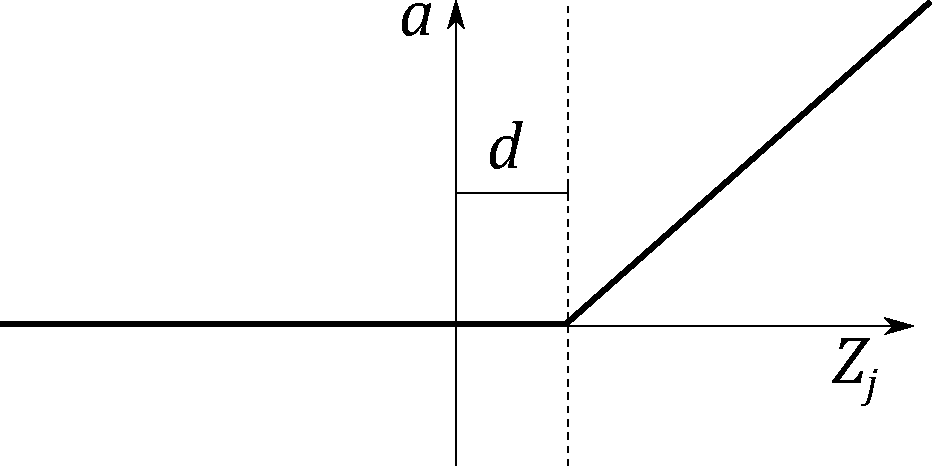
\includegraphics[width=0.5\linewidth]{images/relu.pdf}

%     \caption{In figure captions, explain what the reader is looking at: ``A schematic of the rectifying linear unit, where $a$ is the output amplitude,
%     $d$ is a configurable dead-zone, and $Z_j$ is the input signal'', as well as why the reader is looking at this:
%     ``It is notable that there is no activation \emph{at all} below 0, which explains our initial results.''
%     \textbf{Use vector image formats (.pdf) where possible}. Size figures appropriately, and do not make them over-large or too small to read.
%     }

%     % use the notation fig:name to cross reference a figure
%     \label{fig:relu}
% \end{figure}


% \begin{figure}
%     \centering
%     \begin{subfigure}[b]{0.45\textwidth}
%         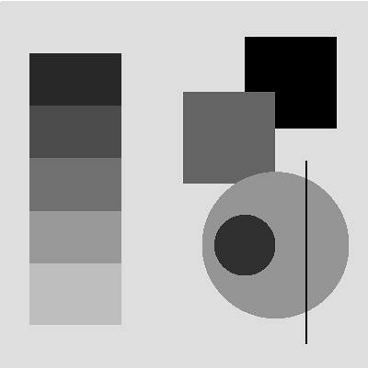
\includegraphics[width=\textwidth]{images/synthetic.png}
%         \caption{Synthetic image, black on white.}
%         \label{fig:syn1}
%     \end{subfigure}
%     ~ %add desired spacing between images, e. g. ~, \quad, \qquad, \hfill etc.
%       %(or a blank line to force the subfigure onto a new line)
%     \begin{subfigure}[b]{0.45\textwidth}
%         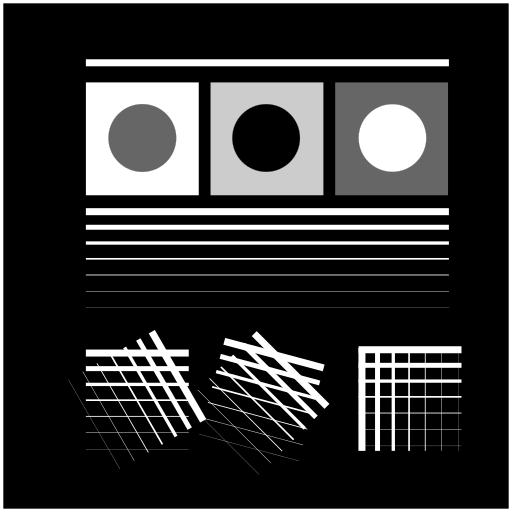
\includegraphics[width=\textwidth]{images/synthetic_2.png}
%         \caption{Synthetic image, white on black.}
%         \label{fig:syn2}
%     \end{subfigure}
%     ~ %add desired spacing between images, e. g. ~, \quad, \qquad, \hfill etc.
%     %(or a blank line to force the subfigure onto a new line)
%     \caption{Synthetic test images for edge detection algorithms. \subref{fig:syn1} shows various gray levels that require an adaptive algorithm. \subref{fig:syn2}
%     shows more challenging edge detection tests that have crossing lines. Fusing these into full segments typically requires algorithms like the Hough transform.
%     This is an example of using subfigures, with \texttt{subref}s in the caption.
%     }\label{fig:synthetic}
% \end{figure}

% \clearpage

% \subsection{Equations}

% Equations should be typeset correctly and precisely. Make sure you get parenthesis sizing correct, and punctuate equations correctly
% (the comma is important and goes \textit{inside} the equation block). Explain any symbols used clearly if not defined earlier.

% For example, we might define:
% \begin{equation}
%     \hat{f}(\xi) = \frac{1}{2}\left[ \int_{-\infty}^{\infty} f(x) e^{2\pi i x \xi} \right],
% \end{equation}
% where $\hat{f}(\xi)$ is the Fourier transform of the time domain signal $f(x)$.

% \subsection{Algorithms}
% Algorithms can be set using \texttt{algorithm2e}, as in Algorithm \ref{alg:metropolis}.

% % NOTE: line ends are denoted by \; in algorithm2e
% \begin{algorithm}
%     \DontPrintSemicolon
%     \KwData{$f_X(x)$, a probability density function returing the density at $x$.\; $\sigma$ a standard deviation specifying the spread of the proposal distribution.\;
%     $x_0$, an initial starting condition.}
%     \KwResult{$s=[x_1, x_2, \dots, x_n]$, $n$ samples approximately drawn from a distribution with PDF $f_X(x)$.}
%     \Begin{
%         $s \longleftarrow []$\;
%         $p \longleftarrow f_X(x)$\;
%         $i \longleftarrow 0$\;
%         \While{$i < n$}
%         {
%             $x^\prime \longleftarrow \mathcal{N}(x, \sigma^2)$\;
%             $p^\prime \longleftarrow f_X(x^\prime)$\;
%             $a \longleftarrow \frac{p^\prime}{p}$\;
%             $r \longleftarrow U(0,1)$\;
%             \If{$r<a$}
%             {
%                 $x \longleftarrow x^\prime$\;
%                 $p \longleftarrow f_X(x)$\;
%                 $i \longleftarrow i+1$\;
%                 append $x$ to $s$\;
%             }
%         }
%     }

% \caption{The Metropolis-Hastings MCMC algorithm for drawing samples from arbitrary probability distributions,
% specialised for normal proposal distributions $q(x^\prime|x) = \mathcal{N}(x, \sigma^2)$. The symmetry of the normal distribution means the acceptance rule takes the simplified form.}\label{alg:metropolis}
% \end{algorithm}

% \subsection{Tables}

% If you need to include tables, like Table \ref{tab:operators}, use a tool like https://www.tablesgenerator.com/ to generate the table as it is
% extremely tedious otherwise.

% \begin{table}[]
%     \caption{The standard table of operators in Python, along with their functional equivalents from the \texttt{operator} package. Note that table
%     captions go above the table, not below. Do not add additional rules/lines to tables. }\label{tab:operators}
%     %\tt
%     \rowcolors{2}{}{gray!3}
%     \begin{tabular}{@{}lll@{}}
%     %\toprule
%     \textbf{Operation}    & \textbf{Syntax}                & \textbf{Function}                            \\ %\midrule % optional rule for header
%     Addition              & \texttt{a + b}                          & \texttt{add(a, b)}                                    \\
%     Concatenation         & \texttt{seq1 + seq2}                    & \texttt{concat(seq1, seq2)}                           \\
%     Containment Test      & \texttt{obj in seq}                     & \texttt{contains(seq, obj)}                           \\
%     Division              & \texttt{a / b}                          & \texttt{div(a, b) }  \\
%     Division              & \texttt{a / b}                          & \texttt{truediv(a, b) } \\
%     Division              & \texttt{a // b}                         & \texttt{floordiv(a, b)}                               \\
%     Bitwise And           & \texttt{a \& b}                         & \texttt{and\_(a, b)}                                  \\
%     Bitwise Exclusive Or  & \texttt{a \textasciicircum b}           & \texttt{xor(a, b)}                                    \\
%     Bitwise Inversion     & \texttt{$\sim$a}                        & \texttt{invert(a)}                                    \\
%     Bitwise Or            & \texttt{a | b}                          & \texttt{or\_(a, b)}                                   \\
%     Exponentiation        & \texttt{a ** b}                         & \texttt{pow(a, b)}                                    \\
%     Identity              & \texttt{a is b}                         & \texttt{is\_(a, b)}                                   \\
%     Identity              & \texttt{a is not b}                     & \texttt{is\_not(a, b)}                                \\
%     Indexed Assignment    & \texttt{obj{[}k{]} = v}                 & \texttt{setitem(obj, k, v)}                           \\
%     Indexed Deletion      & \texttt{del obj{[}k{]}}                 & \texttt{delitem(obj, k)}                              \\
%     Indexing              & \texttt{obj{[}k{]}}                     & \texttt{getitem(obj, k)}                              \\
%     Left Shift            & \texttt{a \textless{}\textless b}       & \texttt{lshift(a, b)}                                 \\
%     Modulo                & \texttt{a \% b}                         & \texttt{mod(a, b)}                                    \\
%     Multiplication        & \texttt{a * b}                          & \texttt{mul(a, b)}                                    \\
%     Negation (Arithmetic) & \texttt{- a}                            & \texttt{neg(a)}                                       \\
%     Negation (Logical)    & \texttt{not a}                          & \texttt{not\_(a)}                                     \\
%     Positive              & \texttt{+ a}                            & \texttt{pos(a)}                                       \\
%     Right Shift           & \texttt{a \textgreater{}\textgreater b} & \texttt{rshift(a, b)}                                 \\
%     Sequence Repetition   & \texttt{seq * i}                        & \texttt{repeat(seq, i)}                               \\
%     Slice Assignment      & \texttt{seq{[}i:j{]} = values}          & \texttt{setitem(seq, slice(i, j), values)}            \\
%     Slice Deletion        & \texttt{del seq{[}i:j{]}}               & \texttt{delitem(seq, slice(i, j))}                    \\
%     Slicing               & \texttt{seq{[}i:j{]}}                   & \texttt{getitem(seq, slice(i, j))}                    \\
%     String Formatting     & \texttt{s \% obj}                       & \texttt{mod(s, obj)}                                  \\
%     Subtraction           & \texttt{a - b}                          & \texttt{sub(a, b)}                                    \\
%     Truth Test            & \texttt{obj}                            & \texttt{truth(obj)}                                   \\
%     Ordering              & \texttt{a \textless b}                  & \texttt{lt(a, b)}                                     \\
%     Ordering              & \texttt{a \textless{}= b}               & \texttt{le(a, b)}                                     \\
%     % \bottomrule
%     \end{tabular}
%     \end{table}
% \subsection{Code}

% Avoid putting large blocks of code in the report (more than a page in one block, for example). Use syntax highlighting if possible, as in Listing \ref{lst:callahan}.

% \begin{lstlisting}[language=python, float, caption={The algorithm for packing the $3\times 3$ outer-totalistic binary CA successor rule into a
%     $16\times 16\times 16\times 16$ 4 bit lookup table, running an equivalent, notionally 16-state $2\times 2$ CA.}, label=lst:callahan]
%     def create_callahan_table(rule="b3s23"):
%         """Generate the lookup table for the cells."""
%         s_table = np.zeros((16, 16, 16, 16), dtype=np.uint8)
%         birth, survive = parse_rule(rule)

%         # generate all 16 bit strings
%         for iv in range(65536):
%             bv = [(iv >> z) & 1 for z in range(16)]
%             a, b, c, d, e, f, g, h, i, j, k, l, m, n, o, p = bv

%             # compute next state of the inner 2x2
%             nw = apply_rule(f, a, b, c, e, g, i, j, k)
%             ne = apply_rule(g, b, c, d, f, h, j, k, l)
%             sw = apply_rule(j, e, f, g, i, k, m, n, o)
%             se = apply_rule(k, f, g, h, j, l, n, o, p)

%             # compute the index of this 4x4
%             nw_code = a | (b << 1) | (e << 2) | (f << 3)
%             ne_code = c | (d << 1) | (g << 2) | (h << 3)
%             sw_code = i | (j << 1) | (m << 2) | (n << 3)
%             se_code = k | (l << 1) | (o << 2) | (p << 3)

%             # compute the state for the 2x2
%             next_code = nw | (ne << 1) | (sw << 2) | (se << 3)

%             # get the 4x4 index, and write into the table
%             s_table[nw_code, ne_code, sw_code, se_code] = next_code

%         return s_table

% \end{lstlisting}

% %==================================================================================================================================
% \chapter{Evaluation}
% How good is your solution? How well did you solve the general problem, and what evidence do you have to support that?

% \section{Guidance}
% \begin{itemize}
%     \item
%         Ask specific questions that address the general problem.
%     \item
%         Answer them with precise evidence (graphs, numbers, statistical
%         analysis, qualitative analysis).
%     \item
%         Be fair and be scientific.
%     \item
%         The key thing is to show that you know how to evaluate your work, not
%         that your work is the most amazing product ever.
% \end{itemize}

% \section{Evidence}
% Make sure you present your evidence well. Use appropriate visualisations, reporting techniques and statistical analysis, as appropriate.

% If you visualise, follow the basic rules, as illustrated in Figure \ref{fig:boxplot}:
% \begin{itemize}
% \item Label everything correctly (axis, title, units).
% \item Caption thoroughly.
% \item Reference in text.
% \item \textbf{Include appropriate display of uncertainty (e.g. error bars, Box plot)}
% \item Minimize clutter.
% \end{itemize}

% See the file \texttt{guide\_to\_visualising.pdf} for further information and guidance.

% \begin{figure}
%     \centering
%     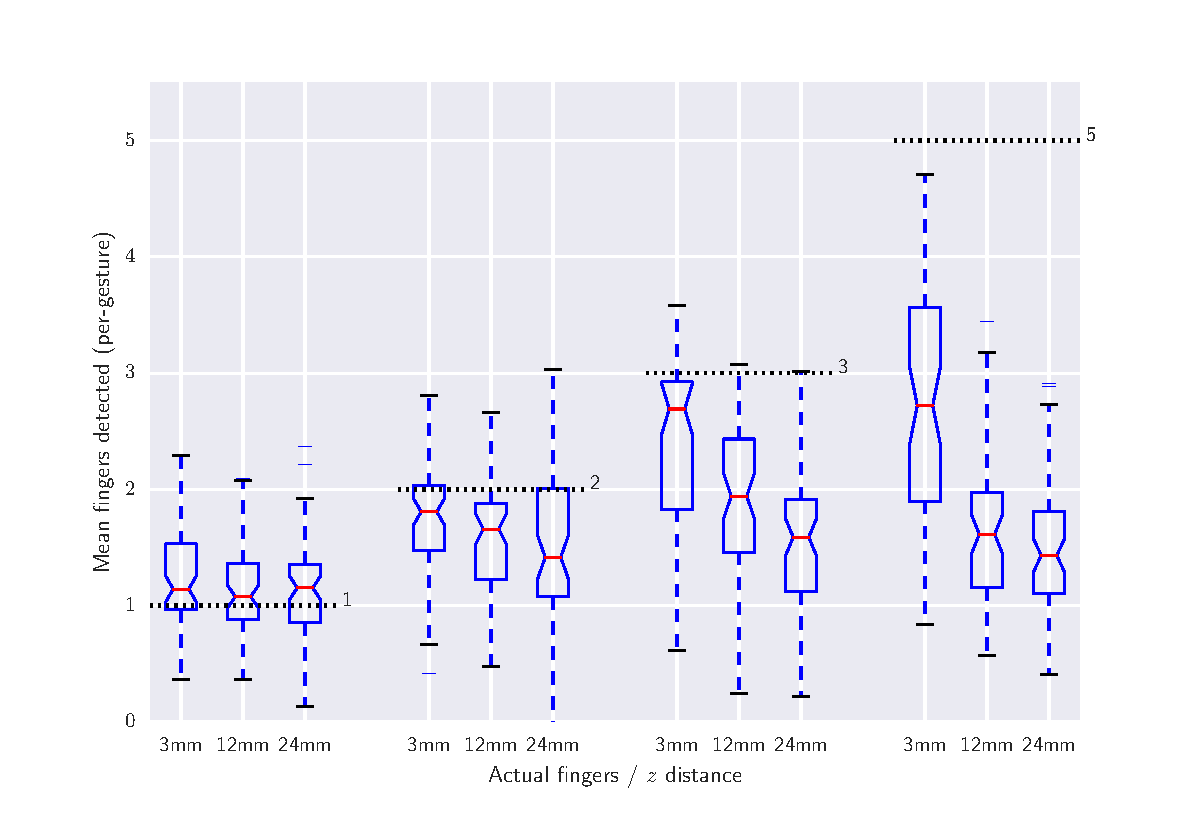
\includegraphics[width=1.0\linewidth]{images/boxplot_finger_distance.pdf}

%     \caption{Average number of fingers detected by the touch sensor at different heights above the surface, averaged over all gestures. Dashed lines indicate
%     the true number of fingers present. The Box plots include bootstrapped uncertainty notches for the median. It is clear that the device is biased toward
%     undercounting fingers, particularly at higher $z$ distances.
%     }

%     % use the notation fig:name to cross reference a figure
%     \label{fig:boxplot}
% \end{figure}


% %==================================================================================================================================
% \chapter{Conclusion}
% Summarise the whole project for a lazy reader who didn't read the rest (e.g. a prize-awarding committee).
% \section{Guidance}
% \begin{itemize}
%     \item
%         Summarise briefly and fairly.
%     \item
%         You should be addressing the general problem you introduced in the
%         Introduction.
%     \item
%         Include summary of concrete results (``the new compiler ran 2x
%         faster'')
%     \item
%         Indicate what future work could be done, but remember: \textbf{you
%         won't get credit for things you haven't done}.
% \end{itemize}

% %==================================================================================================================================
% %
% %
% %==================================================================================================================================
% %  APPENDICES

\begin{appendices}

    \chapter{Appendices}

    \section{Initial Wireframes For Requirement Gathering}
    \label{app:initial_wireframes}

    \begin{figure}
        \centering
        \includegraphics[width=0.95\linewidth]{images/initial_wireframe_1.png}

        \caption{Feature-Full Wireframe}

        % use the notation fig:name to cross reference a figure
        \label{fig:intial_wireframe_1}
    \end{figure}


    \begin{figure}
        \centering
        \includegraphics[width=0.95\linewidth]{images/initial_wireframe_2.png}

        \caption{Simple Wireframe}

        % use the notation fig:name to cross reference a figure
        \label{fig:intial_wireframe_2}
    \end{figure}


    \begin{figure}
        \centering
        \includegraphics[width=0.95\linewidth]{images/initial_wireframe_3.png}

        \caption{Novel-Feature Wireframe}

        % use the notation fig:name to cross reference a figure
        \label{fig:intial_wireframe_3}
    \end{figure}


    % Typical inclusions in the appendices are:

    % \begin{itemize}
    % \item
    %   Copies of ethics approvals (required if obtained)
    % \item
    %   Copies of questionnaires etc. used to gather data from subjects.
    % \item
    %   Extensive tables or figures that are too bulky to fit in the main body of
    %   the report, particularly ones that are repetitive and summarised in the body.

    % \item Outline of the source code (e.g. directory structure), or other architecture documentation like class diagrams.

    % \item User manuals, and any guides to starting/running the software.

    % \end{itemize}

    % \textbf{Don't include your source code in the appendices}. It will be
    % submitted separately.

    \end{appendices}


% \begin{appendices}

% \chapter{Appendices}


% \section{}

% % Typical inclusions in the appendices are:

% % \begin{itemize}
% % \item
% %   Copies of ethics approvals (required if obtained)
% % \item
% %   Copies of questionnaires etc. used to gather data from subjects.
% % \item
% %   Extensive tables or figures that are too bulky to fit in the main body of
% %   the report, particularly ones that are repetitive and summarised in the body.

% % \item Outline of the source code (e.g. directory structure), or other architecture documentation like class diagrams.

% % \item User manuals, and any guides to starting/running the software.

% % \end{itemize}

% % \textbf{Don't include your source code in the appendices}. It will be
% % submitted separately.

% \end{appendices}

%==================================================================================================================================
%   BIBLIOGRAPHY

% The bibliography style is abbrvnat
% The bibliography always appears last, after the appendices.



\bibliographystyle{abbrvnat}

\bibliography{l4proj}

\end{document}
